\section{Results}
\label{sec:results} 

Our work aims to analyze the evolution of the Bitcoin Blockchain on certain
time snapshots. Our data are of a high quality since they are generated from a
controlled environment and hence they do not include any noise. They range from
2009 until the March of 2017 and are approximately 98GBs, which we finally
manage to reduce to 14GBs of parquet files. We perform our computations for
each year individually and we do not count the results of previous years in
order to compute a metric for the next. Our analysis is based on years and
months, however we limit the amount of visualizations in the present manuscript
for reader's-ease reasons. We choose to discuss the results only for the years
as those are sufficient for comparisons and conclusions. In our
website~\cite{website} we provide also visualizations of the results per month
of each year, as well as the graph visualizations of the communities that produced the 
minimum Conductance, hence the Conductance of the whole graph. 


\subsection{Size}
\fref{fig:fig3} represents the evolution of the graph for each year in terms of size. As we refer in~\secref{sec:background} the size of the graph is conducted from the number of edges. Since each edge on the graph represents a transaction, we observe that the transactions continuously rose per year.
For 2009 the number of transactions was 22.000 while for 2015 reached a peak with 4.8 billion.

\begin{figure}[h!]
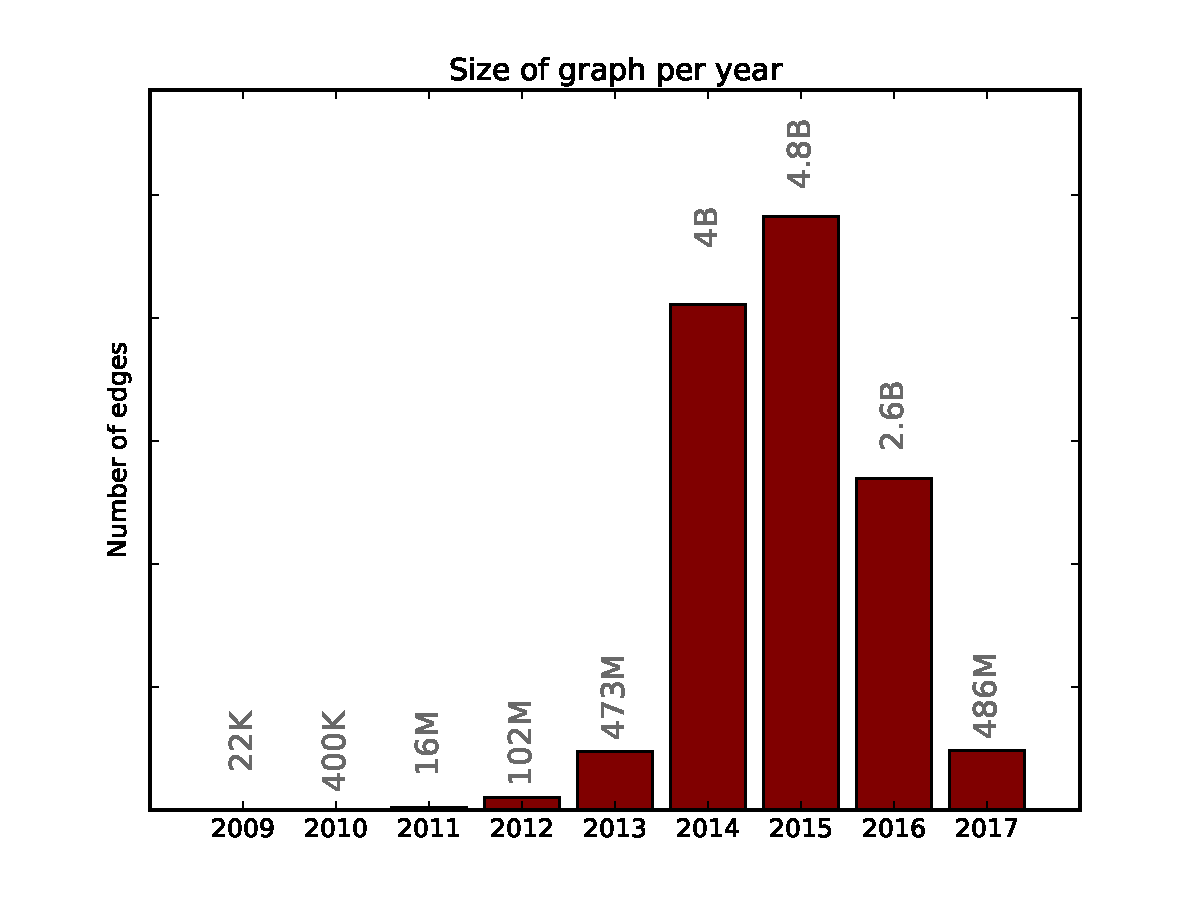
\includegraphics[width=1\linewidth]{./images/size}
\centering
\caption{The size of the graph per year. Since the size is conducted from the number of edges and the edges in the graph represent transactions, we observe that transactions in the Bitcoin Blockchain continuously increased. The peak is in 2015 where 4.8 billion transactions take place.}
\label{fig:fig3}
\end{figure}


\subsection{Triangle Participation Ratio}
\fref{fig:fig4} demonstrates the clustering of the graph through Triangle Participation Ratio. For the years 2009 to 2012 there is a fluctuation which later becomes a constant decrease until the March of 2017 that reaches the half of the value of 2012. We interpret the TPR as transactions between cliques. The decrease of TPR after 2012 was expected due to the size of the graph that starts increasing dramatically, hence the transactions become more spread between users. Generally, we observe that the TPR does not exceed 37\% for any of the years which indicates the lack of small communities compared to the total size of the network.


\begin{figure}[h!]
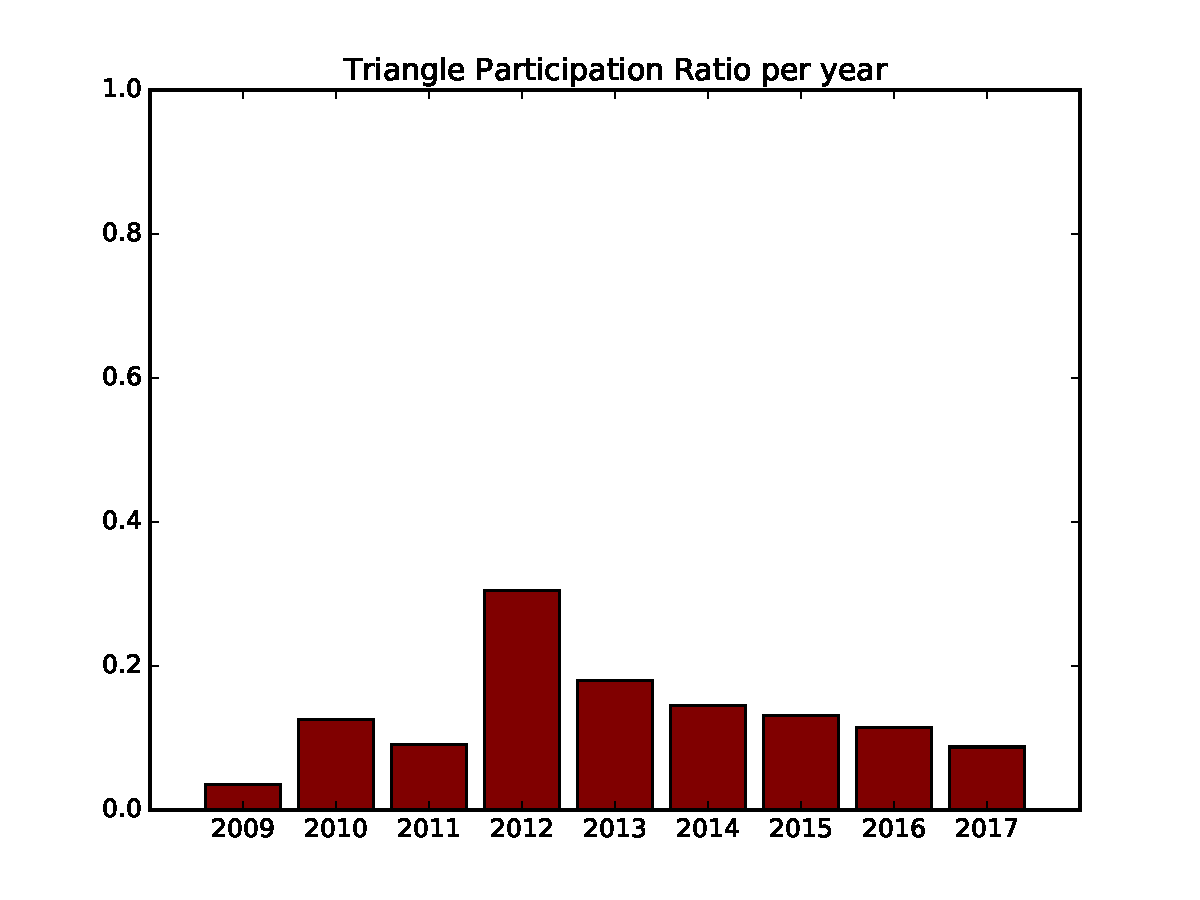
\includegraphics[width=1\linewidth]{./images/tpr}
\centering
\caption{The Triangle Participation Ratio of the vertices for each year from 2009 until March of 2017. From the results we can observe that in general the ratio is pretty low which is interpreted as the difficulty of existance of small societies in a large graph.}
\label{fig:fig4}
\end{figure}

\subsection{Clustering Coefficient}
When we turn to analyze the Clustering Coefficient, as~\fref{fig:fig5} shows,
we can observe that the Average Clustering Coefficient for each year is between
0 and 0.1. This ratio indicates that there are only a few vertices that their
neighbors form a clique and we can correlate it with the low Triangle
Participation Ratio.

On the other hand, the Global Clustering Coefficient has greater values than the Average. The distribution of the ratio is between 0.04 and 0.7 with the second one being a peak in 2011 followed by 2012 with a ratio around 0.65. From those two results we can comprehend that a high number of closed triplets existed in each graph and hence the clustering of those two individual years was very good compared to others. However, as a general conclusion most of the years do not have a good clustering between transactions.

\begin{figure}[t]
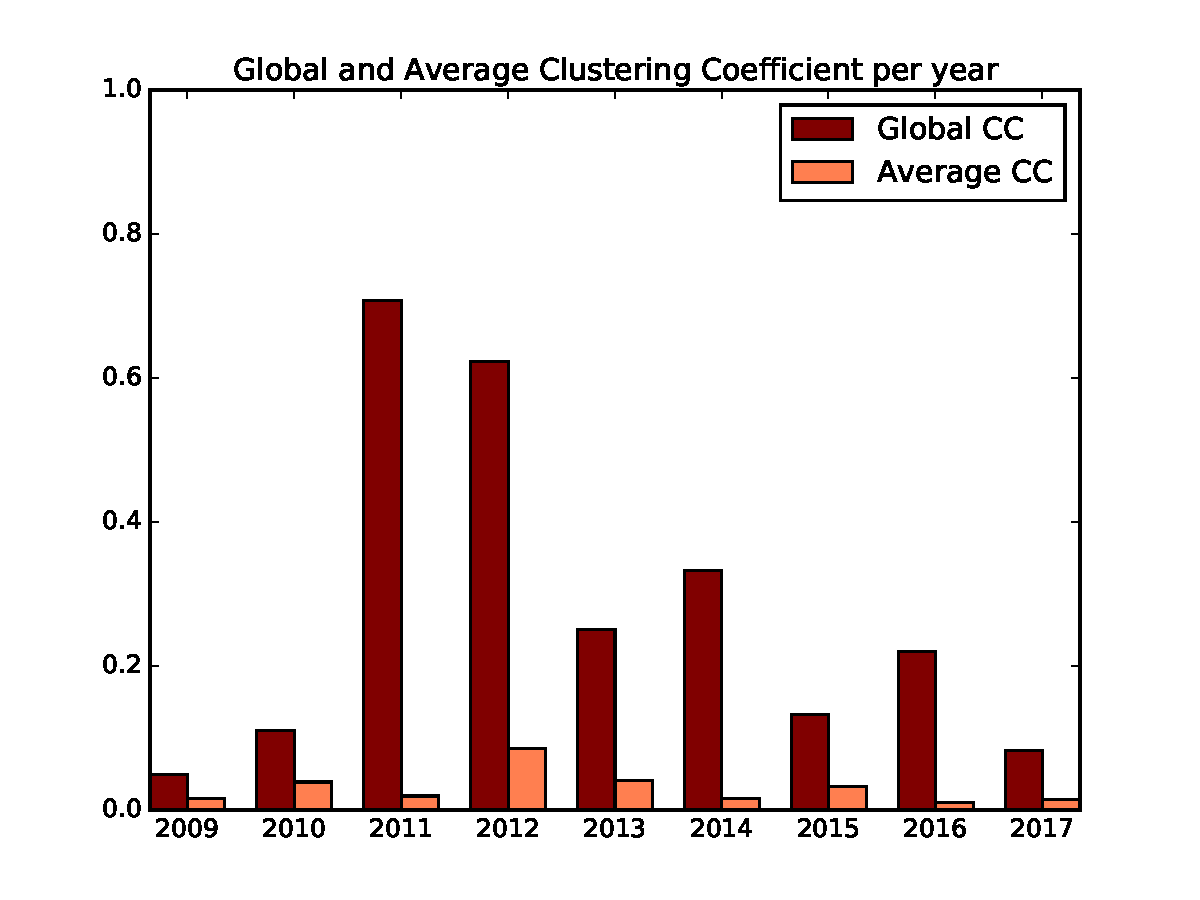
\includegraphics[width=1\linewidth]{./images/cc}
\centering
\caption{The Global and the Average Clustering Coefficient of the graph for each year from 2009 until March of 2017. The years 2011 and 2012 have the highest ratio as the Global Clustering Coefficient is concerned and hence in those two years there was a good clustering between transactions. However, for most of the years the ratio is low and indicates poor clustering.}
\label{fig:fig5}
\end{figure}


\subsection{Conductance}
~\fref{fig:fig6} demonstrates the Conductance of the graph for the years 2009 until 2017 while
~\fref{fig:fig7} represents the number of edges of the selected communities proportional to the total number of edges of the graph. 
As we can observe, the first two years of the existance
of the Bitcoin Blockchain have the highest ratio. Specifically,
for 2009 the ratio exceeds 0.9 and for 2010 it is almost 0.7. That indicates
that those two years the communities are not very well isolated and that there are more outward connections 
for any cluster of vertices. On the other
hand, the years 2012 and 2013 have the lowest ratio, with the first plunged
below 0.1. Undoubtedly, these two years state how diverse and expansive the
graph is and from technical perspective they imply a more inward-looking cluster. 
Generally, for most of the years the conductace is far below 0.5,
thus the communities tend to be well isolated.


\begin{figure}[h!]
    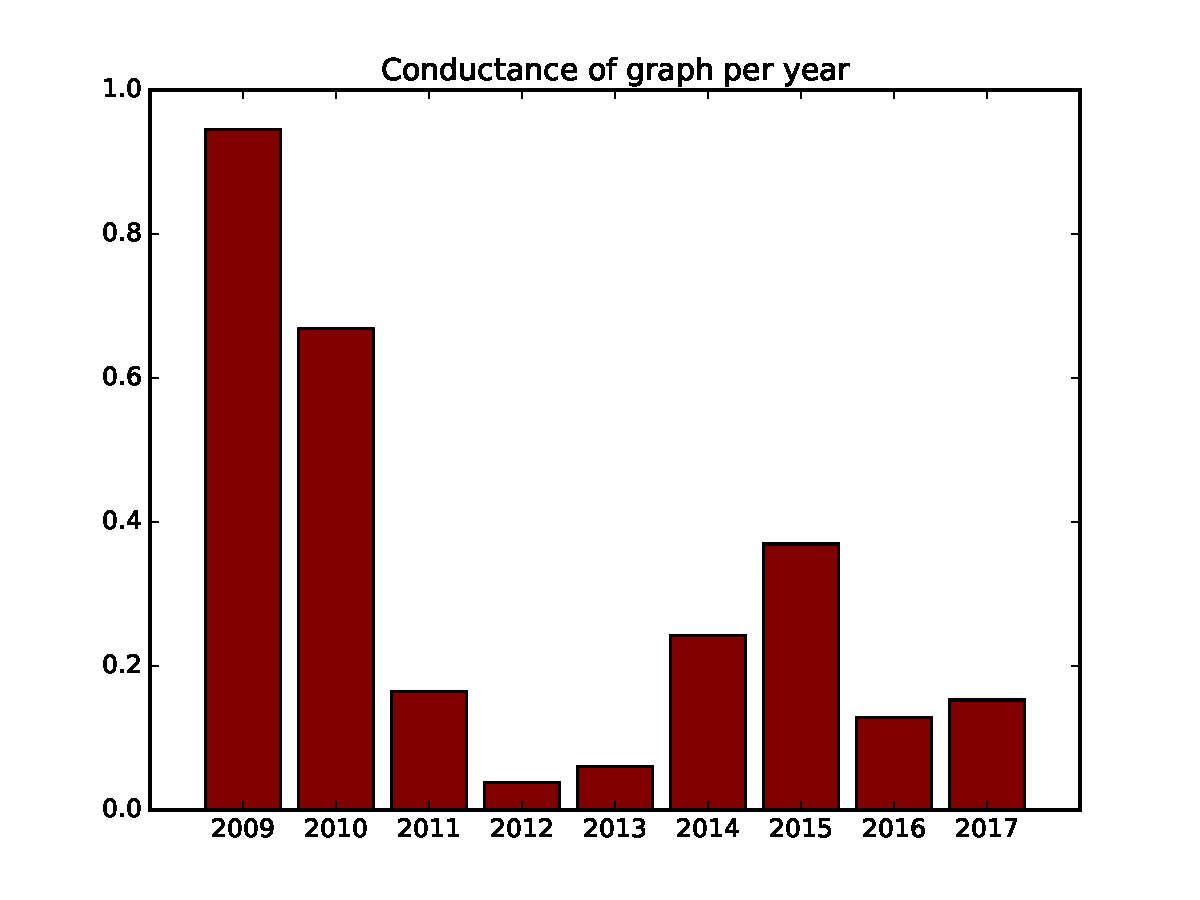
\includegraphics[width=1\linewidth]{./images/conductance}
	\centering
	\caption{The Conductance of 10 communities of the graph for each year from 2009 until March of 2017. The years 2009 and 2010 have the highest ratio thus in those two years the graph was not well isolated and had some bottleneck. The years 2012 and 2013 show that the graph was diverse. In general for most of the years the conductance is far below the half which is a sign of good clustering.}
	\label{fig:fig6}
\end{figure}

\begin{figure}[h!]
    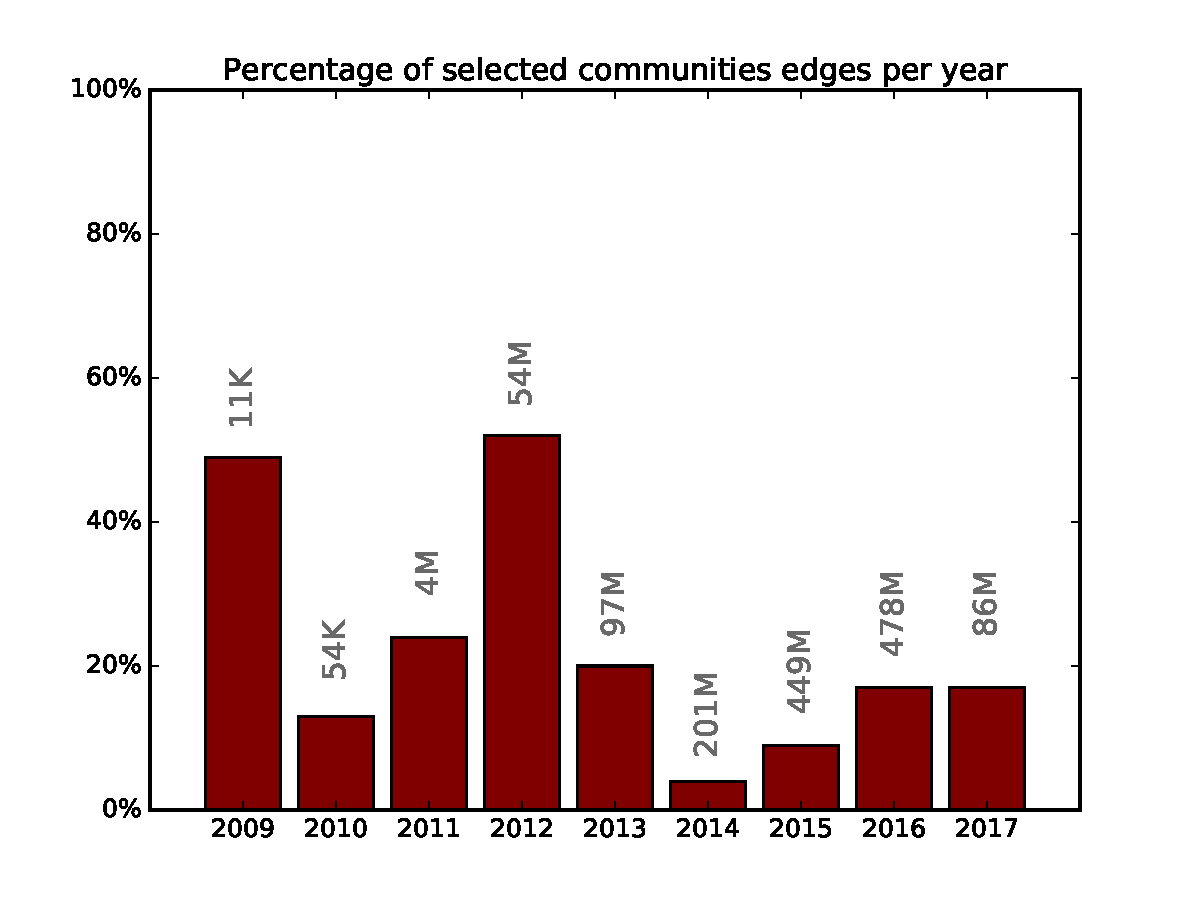
\includegraphics[width=1\linewidth]{./images/edgePercentage}
	\centering
	\caption{To compute conductance we select the top 10 communities with the highest number of edges. The chart shows the percentage and the number of the selected edges of the communities proportional to the total edges of the graph for each year from 2009 to March 2017.}
	\label{fig:fig7}
\end{figure}





\subsection{Bridge Ratio and Diameter}
As we further discuss later in~\secref{sec:discussion}, our computations are
heavy and as the size of the graph increases the more trivial it becomes to
obtain a result, especially for the Bridge Ratio and the Diameter. Hence, we
are not able to have a complete image as those metrics are concerned. 

For the Bridge Ratio we are able to obtain a result only for 2009 as an annual image and for 2009-2010 for the months. The reported result for 2009 is that 24\% of the edges are bridges, however we cannot reach to any conclusion. As the Diameter is concerned, the result that we obtain for both years and months is for 2009, which is \textit{Infinity} in both cases and the meaning is that the graph has disconnected components.


